\documentclass[12pt]{report}
\usepackage{graphicx}
\usepackage{amsmath}
\usepackage{amsfonts}
\usepackage{amssymb}
\usepackage{algorithm}
\usepackage{algorithmic}
\usepackage{hyperref}
\usepackage{cite}
\usepackage{longtable}
\usepackage{array}
\sloppy
\title{Multi-objective Evolutionary Algorithms for Solving the Electric Vehicle Charging Station Infrastructure Problem}
\author{Harith Elamin}
\date{May 2025}
\begin{document}

% Title Page
\maketitle

% Table of Contents
\tableofcontents
\newpage

% List of Figures
\listoffigures
\newpage

\begin{abstract}
The growing awareness among people, including governments and individuals, of the risks posed by the pollution of gasoline and diesel vehicle emissions has contributed significantly to the shift toward clean energy for both public and private transport. Efficient and accessible transportation is a critical challenge that affects urban planners and corporate decision makers. Significant investments in technology and infrastructure are necessary to ensure that sufficient charging stations are available in strategic locations. This is crucial to ensure a successful transition to sustainable electric transport.

This thesis explores the use of the multi-objective evolutionary algorithm to optimize the placement and configuration of electric vehicle charging stations (EVCS). The goal is to find a solution that maximizes the geographic area covered by EV charging stations, minimizes the cost of setting up the infrastructure, and maximizes the power level of the stations to improve charging efficiency and reduce waiting times. By applying MOOP, such as the NSGA-II algorithm, we demonstrate the potential of evolutionary algorithms to address the complexities of EV charging station layout in an urban environment. The results show that NSGA-II provides an efficient and versatile solution to the challenges of the electric vehicle charging station infrastructure.
\end{abstract}

\chapter{Introduction}
The rapid expansion of electric vehicle adoption presents both an opportunity and a challenge for urban transport systems. Electric vehicles have the potential to reduce air pollution and the use of conventional fuels such as diesel and gasoline, but their widespread use requires the establishment of a reliable and accessible charging infrastructure.

Selecting the location of electric vehicle charging stations is a complex problem that involves balancing several conflicting objectives. As electric vehicle adoption continues to increase worldwide, establishing reliable, efficient, and accessible infrastructure is becoming increasingly important. A key challenge in this process is to identify the optimal locations for charging stations to meet the needs of electric vehicle users while minimizing associated costs and covering as much area as possible to ensure connectivity.

Minimizing overall infrastructure costs an important goal when selecting the location of charging stations. This includes both direct costs, such as installing and maintaining charging stations, and the costs of users accessing those stations. Reducing costs is a critical aspect of urban planning, so it is essential to ensure that charging stations are strategically distributed to keep costs low while still meeting demand. Efficient distribution plays a key role in balancing affordability and user accessibility.

In addition to cost considerations, another important factor in determining the location of EV charging stations is minimizing the travel distance for EV users. The availability of charging stations directly affects the possibility of using EVs. Stations should be strategically placed, whether in densely populated urban areas or rural areas where access to charging infrastructure may be limited. Reducing the distance that drivers have to travel to find a charging point is crucial as it enhances the desire of drivers to use EVs. Conversely, long waits at charging stations or difficulty finding a nearby station can be a reason for drivers to avoid using EVs altogether.

Furthermore, the power level of the chargers should be considered to minimize the charging time. By optimizing the charging power of each station, the overall efficiency of the network can be improved, resulting in faster charging times and a better user experience. This consideration is crucial in ensuring that the charging infrastructure meets the growing demand for electric vehicles while minimizing user waiting times.

Moreover, traditional approaches to solving the EVCS location problem typically rely on optimization techniques such as mathematical programming. This approach often focuses on single-objective optimization, where only one aspect of the problem is prioritized, such as minimizing cost. Although these methods can provide effective solutions in certain scenarios, they often fail when dealing with trade-offs between multiple objectives, such as cost, coverage, and load balancing. In addition, traditional optimization techniques can be computationally expensive and time-consuming, especially when the problem involves large urban areas with many potential charging station locations. Multi-objective optimization techniques, such as multi-objective evolutionary algorithms (MOEAs), have emerged as a promising alternative to address the complexity of the EVCS problem. These algorithms are designed to find a variety of solutions that represent different trade-offs between competing objectives. By incorporating multiple objectives into the optimization process, multi-objective evolutionary algorithms can provide decision makers with a broader set of possible solutions, allowing them to choose the solution that best meets the needs of society while balancing the different costs and benefits of charging station placement. These methods are particularly useful when dealing with real-world problems that require the simultaneous optimization of multiple, often conflicting, objectives. In short, locating electric vehicle charging stations is a complex task that involves addressing different objectives, such as maximizing coverage,  and maximizing the power of the charger to reduce waiting time. Traditional methods may not be sufficient to handle competing objectives, making multi-objective evolutionary algorithms an attractive solution for optimizing EV charging infrastructure placement.
\section{Motivation}
The transition to electric vehicles is a key component of sustainable transportation systems, addressing growing concerns about air pollution, climate change, and reliance on conventional fuels such as gasoline and diesel. As EV adoption continues to rise, one of the most pressing challenges is developing an efficient, widely available, and accessible electric vehicle charging station (EVCS) infrastructure. The success of this transition depends largely on optimizing the placement, configuration, and capacity of charging stations to meet the needs of both private and public transportation. However, this task is complicated by the multiple conflicting objectives that must be balanced, such as minimizing costs, maximizing coverage, and minimizing charging time.

Traditional optimization methods are often inadequate to solve such multidimensional problems. This is where multi-objective evolutionary algorithms (MOEAs), such as NSGA-II, come in. These algorithms are well-suited to handling the complexities of EVCS infrastructure optimization due to their ability to search for solutions that simultaneously meet multiple objectives.

The motivation behind this thesis stems from the need to explore advanced optimization techniques such as MOEAs to address the pressing challenges faced by urban planners and decision makers in the field of electric vehicle charging infrastructure. As the number of electric vehicles grows, the need for a strong charging network increases. The placement and configuration of electric vehicle charging stations must ensure adequate coverage across urban areas, while minimizing infrastructure costs. 

Furthermore, this research aims to demonstrate how evolutionary algorithms, especially NSGA-II, can provide efficient and scalable solutions to these challenges, contributing to the creation of a sustainable and efficient electric vehicle charging infrastructure.

\section{Problem Definition}
The rapid trend of governments to push for electric vehicles has created an urgent need for a strong and widespread electric vehicle charging infrastructure. Ensuring that electric vehicle charging stations are optimally distributed across geographies with high capacity and cost-effectiveness to meet the needs of electric vehicle users is a complex challenge. The problem is complex, involving a number of objectives, such as increasing coverage area, minimizing costs, and reducing waiting time. This research focuses on leveraging multi-objective evolutionary algorithms to address these objectives and find optimal solutions for the deployment of electric vehicle charging infrastructure. The problem can be formalized as follows:
\begin{itemize}
    \item Coverage: The goal is to increase the geographical area covered by electric vehicle charging stations, as the good distribution of electric vehicle charging stations allows electric vehicle owners to easily access these stations, which reduces time and effort.
    
    \item Chargers Power Level: Charger power level: The efficiency of charging stations plays an important role in charging electric vehicles, as it affects the speed of the charging process. Charging stations with high capacity reduce charging time, which leads to less waiting time for users. In addition, reducing charging time enhances the user experience and increases the efficiency of the network in general. It is necessary to provide charging stations capable of handling high power requirements to meet the growing needs of electric vehicles.
    
    \item Reducing the number of stations: Reducing the number of charging stations without compromising network coverage is critical to reducing costs and improving operational efficiency. Balancing station location with network coverage ensures adequate coverage of the service area while minimizing infrastructure costs.
    
    \item Reducing the number of chargers: In addition to reducing the number of charging stations, it is also necessary to reduce the number of individual chargers at each station. This helps reduce initial investment and operating costs while maintaining service levels and user convenience.

        
    \item Cost: Reducing the cost of building electric charging stations is of great importance to decision makers. The balance between comprehensive coverage and affordability is a key element of the optimization problem, but deploying a large number of charging stations across a large area can be very expensive.
\end{itemize}

\section{Objective of the Thesis}
This thesis aims to:
\begin{itemize}
    \item Investigating multi-objective evolution algorithms (MOEAs) to solve the EVCS infrastructure problem.
    \item Optimizing multiple objectives at the same time, including infrastructure cost, coverage, and power levels per charging stand.
    \item Comparing the results obtained from the application of the genetic algorithm with those found in the literature review.
    \item Presenting the results from the research thesis experiments and analyzing their performance.
\end{itemize}


\chapter{Literature Review}

\section{Electric Vehicle Charging Station Infrastructure}
The problem of determining optimal EVCS locations has been the focus of several studies. Early research focused on single-objective optimization techniques, primarily aimed at minimizing costs \cite{ref1}. However, as the number of electric vehicles increases, it has become clear that reducing costs alone is not enough to meet users' needs. Therefore, multi-objective optimization techniques can be used to solve complex problems with multiple conflicting objectives, as they optimize multiple criteria at the same time.

Recent work has explored various approaches to solve this problem, including:
\begin{itemize}
    \item \textbf{Mathematical methods}: These methods use linear, and nonlinear programming to model and solve the placement and sizing problem, often assuming a fixed demand \cite{ref2}.
    \item \textbf{Genetic algorithm technique}: Genetic algorithms, simulated annealing, and particle swarm optimization have been used to optimize the locations of charging stations \cite{ref3}.
    \item \textbf{Evolutionary algorithms}: Multi-objective evolutionary algorithms (MOEAs) have become increasingly popular due to their ability to handle multiple conflicting objectives simultaneously. Algorithms such as NSGA-II and SPEA2 have been successfully applied to optimize EVCS placement \cite{ref4}.
\end{itemize}

\section{Multi-objective Evolutionary Algorithms}
Multi-objective evolutionary algorithms are a class of algorithms that are designed to solve optimization problems involving more than one objective. Unlike traditional optimization methods, which aim to find a single optimal solution, MOEAs aim to provide a set of diverse solutions that represent different trade-offs among the objectives \cite{ref5}.

One of the most widely used Multi-Objective Evolutionary Algorithms (MOEAs) is:

\begin{itemize}
    \item \textbf{NSGA-II (Non-dominated Sorting Genetic Algorithm II)}: NSGA-II is a fast and efficient algorithm that uses non-dominated sorting, crowding distance, and elitism to preserve diversity in the population. It is well-suited for solving complex multi-objective optimization problems and has been widely adopted in both academic and real-world applications \cite{ref6}.
\end{itemize}

NSGA-II algorithm has been successfully applied across various domains, including engineering design, environmental planning, and transportation systems.


\chapter{Methodology}

\section{Problem Formulation}
The Electric Vehicle Charging Station(EVCS) infrastructure problem can be formulated as a multi-objective optimization problem with the following decision variables:
\begin{itemize}
    \item A set of candidate charging station locations, denoted as $S = \{s_1, s_2, ..., s_n\}$, where each location $s_i$ is defined by its geographic coordinates $(x_i, y_i)$ within the urban area.

    \item  The power level assigned to chargers at each station, denoted as $P_i \in \{11.5, 14.2, 19.2, 25, 60, 62, 80, 120, 150, 180, 200, 240, 250, 300, 325, 350, 400\} $~kW, representing the charging speed selected for station $i$ to reduce user waiting time.

    \item The installation cost associated with each charger, denoted by $C_i$, which reflects the total economic expense of deploying a charger at station $i$, considering infrastructure and equipment costs.

    \item The number of charging stations deployed, denoted by $N_s$, which impacts both installation cost and spatial resource usage.

    \item The total number of chargers installed across all stations, denoted by $N_c$, which also contributes to overall cost and infrastructure requirements.
\end{itemize}


The constraints considered in the optimization model are as follows:
\begin{itemize}
    \item The total number of charging stations deployed ($N_s$) must not exceed a predefined upper limit or budget constraint, ensuring feasibility in terms of infrastructure cost and urban space availability.

    \item The total number of chargers installed at each station must respect the station's physical capacity and grid connection limits, and the aggregate charging demand must not exceed this capacity based on both the number of chargers and their power levels ($P_i$).

    \item Each electric vehicle (EV) must be within an acceptable distance from at least one charging station to ensure adequate spatial coverage and accessibility for all users.

    \item The total installation cost, calculated based on the number and type of chargers deployed ($C_i$), must remain within the available budget or funding constraints.

    \item Charger power levels must be selected from the discrete set $\{50, 150, 250\}$~kW, corresponding to standardized fast-charging options.
\end{itemize}



\section{Multi-objective Evolutionary Algorithm (MOEA) Framework}
We employ the \textbf{NSGA-II} algorithm, which is  is a multi-objective evolutionary algorithm that applies non-dominated sorting to rank solutions into various fronts \cite{ref8}.

Standard genetic operators such as selection, crossover, and mutation are employed within the algorithm. The fitness of each solution is assessed according to the three objectives previously defined: coverage, charger power level per stand, and charger cost.

\chapter{The Experiment}

\begin{figure}[h!]
    \centering
    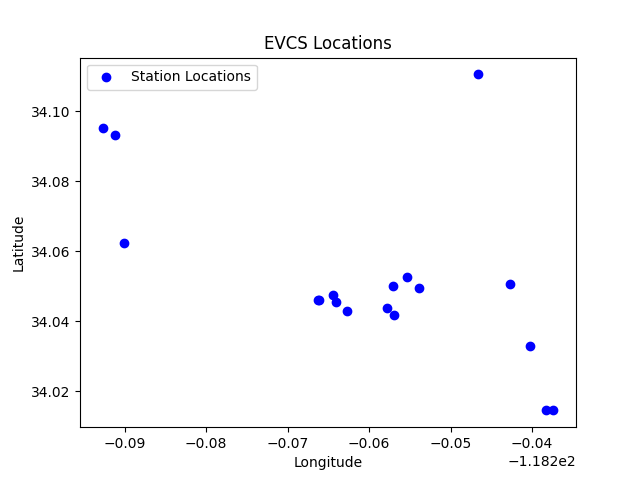
\includegraphics[width=0.8\textwidth]{Figures/original_map.PNG}
    \caption{Origina stations map.}
    \label{fig:original_map}
\end{figure}



\begin{figure}[h!]
    \centering
    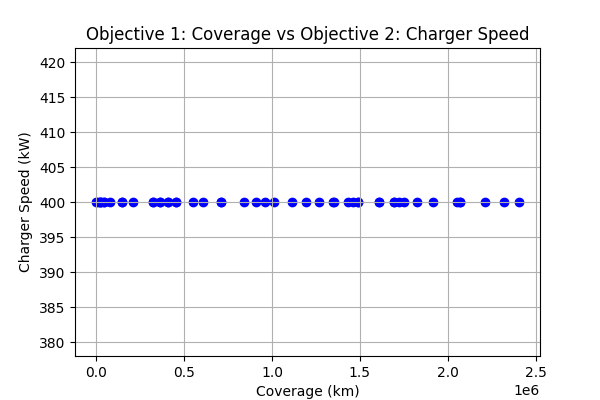
\includegraphics[width=0.8\textwidth]{Figures/Figure_1.png} 
    \caption{Coverage vs Charger speed}
    \label{fig:Coverage vs Charger speed}
\end{figure}




\begin{figure}[h!]
    \centering
    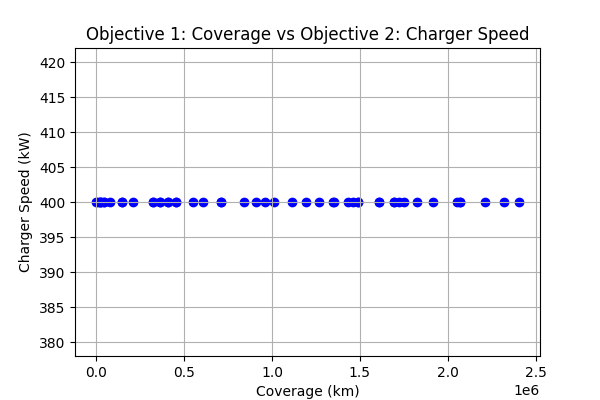
\includegraphics[width=0.8\textwidth]{Figures/Figure_1.png} 
    \caption{Objective 1: Coverage vs Objective 2: Charger speed.}
    \label{fig:your_image_label}
\end{figure}

\begin{table}[h!]
    \centering
    \small % Reduce the font size for the table
    \begin{tabular}{|>{\raggedright\arraybackslash}p{2cm}|>{\raggedright\arraybackslash}p{3cm}|>{\raggedright\arraybackslash}p{2cm}|>{\raggedright\arraybackslash}p{2cm}|>{\raggedright\arraybackslash}p{3cm}|}
    \hline
    \textbf{Power Range} & \textbf{Type of Charger} & \textbf{Hardware Cost} & \textbf{Installation Cost} & \textbf{Total Estimated Cost} \\
    \hline
    3 kW - 7 kW & Level 1 or Level 2 Charger & \$500 - \$1,500 & \$300 - \$500 & \$800 - \$2,000 \\
    \hline
    7 kW - 22 kW & Level 2 Charger & \$1,500 - \$5,000 & \$1,000 - \$2,500 & \$2,500 - \$7,500 \\
    \hline
    50 kW - 100 kW & DC Fast Charger & \$30,000 - \$50,000 & \$50,000 - \$100,000 & \$80,000 - \$150,000 \\
    \hline
    100 kW - 150 kW & DC Fast Charger & \$50,000 - \$70,000 & \$50,000 - \$100,000 & \$100,000 - \$170,000 \\
    \hline
    150 kW - 200 kW & DC Fast Charger & \$70,000 - \$100,000 & \$100,000 - \$150,000 & \$170,000 - \$250,000 \\
    \hline
    200 kW - 350 kW & Ultra-Fast Charger & \$100,000 - \$150,000 & \$150,000 - \$250,000 & \$250,000 - \$400,000 \\
    \hline
    350 kW - 400 kW & Ultra-Fast Charger & \$120,000 - \$150,000 & \$150,000 - \$250,000 & \$270,000 - \$400,000 \\
    \hline
    \end{tabular}
    \caption{Cost Estimates for Different Types of EV Chargers}
    \end{table}
    


\section{Test Case}
In this experiment, we evaluate the performance of NSGA-II algorithm. The test case is based on one of the largest cities in the world, and the details of the test case include:

\begin{itemize}
    \item 100 potential locations for charging stations, each location has number of charger, with 1000 EVs in the area. The dataset includes the following attributes for each location:
    \begin{itemize}
        \item \textbf{Id}: Unique identifier for each charging station location.
        \item \textbf{Coordinates}: The geographical coordinates of each charging station location.
        \item \textbf{Power Level (W)}: The power rating of the chargers at each site, (50 w, 150 w, 250 w).
        \item \textbf{Chargers per Site}: The number of chargers installed at each station.
        \item \textbf{Cost}: The cost associated with installing and operating each charger at the station.
    \end{itemize}
\end{itemize}

In this research on electric vehicle charging stations (EVCS), we selected a California data set due to its leading role in the adoption of electric vehicles and the development of its charging infrastructure. In addition, the installation costs for the chargers were sourced from standard prices used across the United States.

California is among the regions that have implemented EV policies to reduce pollution. Furthermore, California boasts a high population density and a large number of electric vehicles and EV charging stations, providing a rich source of data on usage, location, and other key factors influencing the development of charging stations. This data enhances the potential for EV charging stations to be deployed in other regions.

The NSGA-II algorithm will be applied to optimize the three objectives: coverage, power level per stand, and charging cost.


\section{Performance Metrics}
The performance of the algorithms is evaluated on the following metrics:
\begin{itemize}
    \item \textbf{Pareto Front Coverage}: Measures how well the obtained Pareto front approximates the true Pareto front.
    \item \textbf{Hypervolume Indicator}: Measures the volume dominated by a set of solutions in the objective space, with a larger volume indicating better performance.
    \item \textbf{Convergence and Diversity}: Evaluates the convergence to the Pareto front and the diversity of the solutions.
    \item \textbf{Coverage}: Evaluates how well the area is covered by the selected charging stations. This ensures that the solution minimizes the travel distance for EV users.
    \item \textbf{Power Level per Stand}: Measures the total power requirement for each charging station to meet the demand in the area.
    \item \textbf{Cost of Charger}: Evaluates the total cost involved in setting up each charger, including installation and operational costs.
\end{itemize}

\chapter{Results and Discussion}


\section{Analysis of Results}

\begin{figure}[h!]
    \centering
    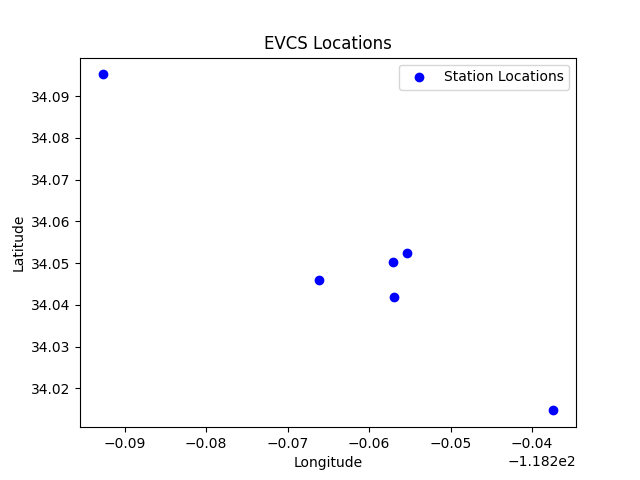
\includegraphics[width=0.8\textwidth]{Figures/optimized_map.PNG}
    \caption{Optimized stations map.}
    \label{fig:original_map}
\end{figure}

\vspace{1cm} %

\begin{figure}[h!]
    \centering
    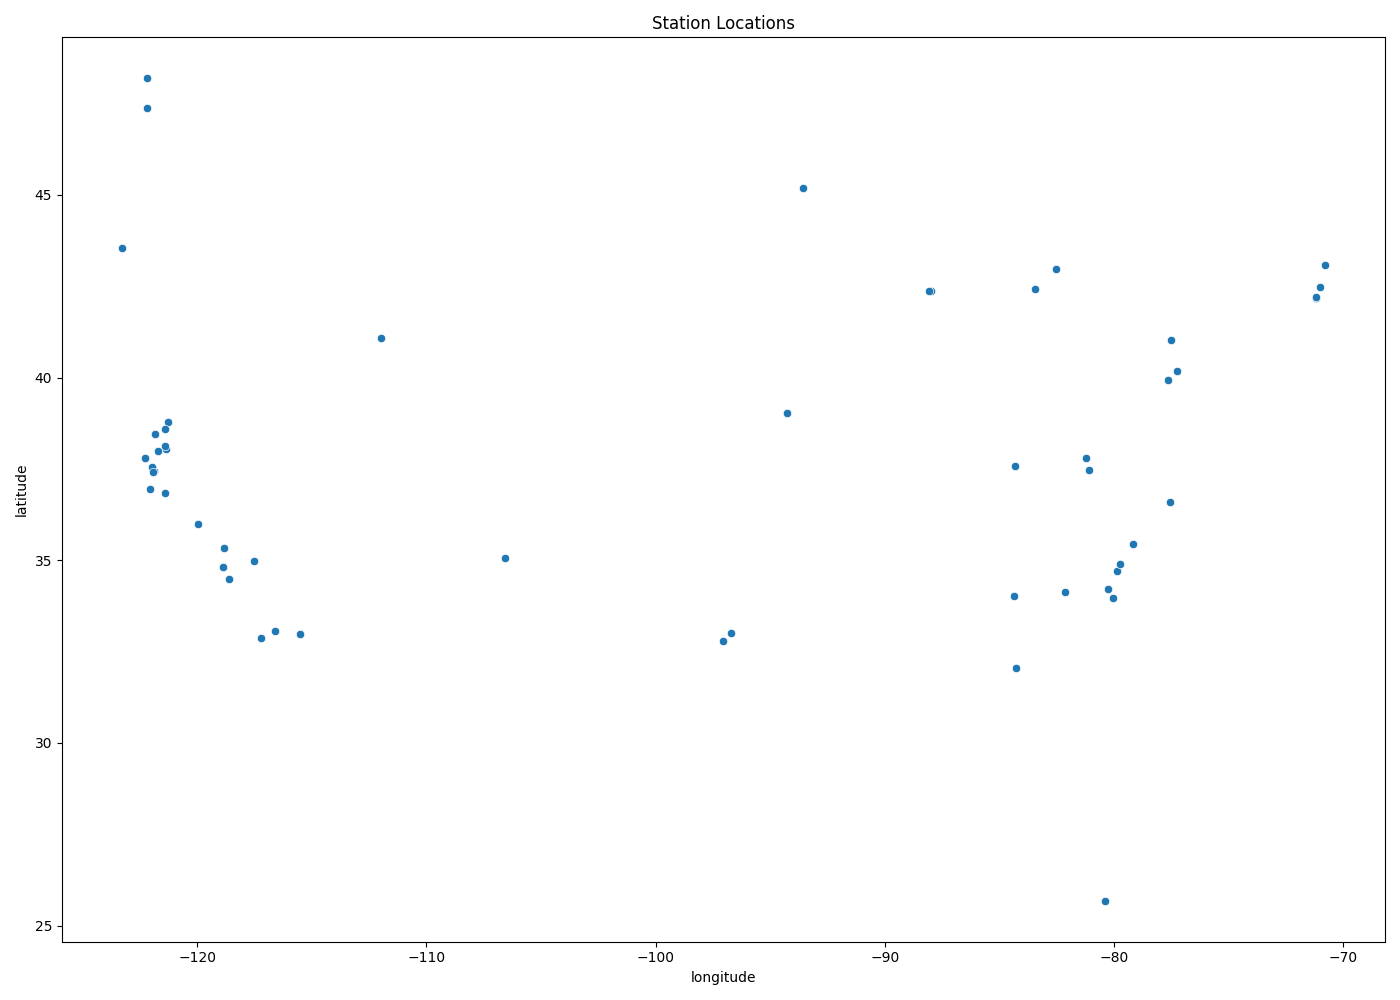
\includegraphics[width=0.8\textwidth]{Figures/station_locations.png}
    \caption{stations locations}
    \label{fig:OOriginal_map}
\end{figure}

\begin{figure}[h!]
    \centering
    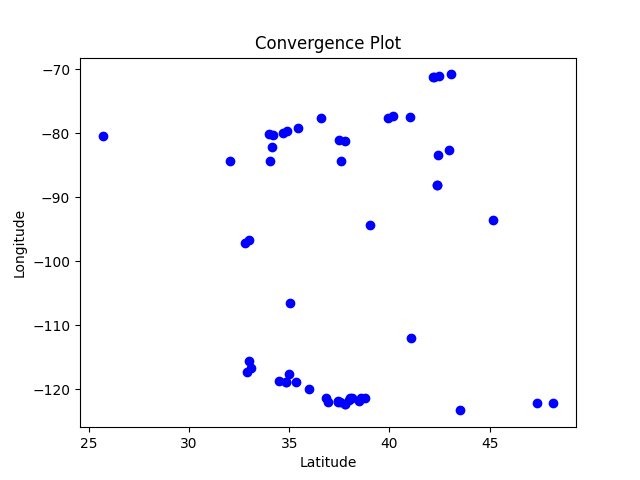
\includegraphics[width=0.8\textwidth]{Figures/convergence_plot.png}
    \caption{stations locations}
    \label{fig:Original_map}
\end{figure}

\vspace{1cm} %

\begin{figure}[h!]
    \centering
    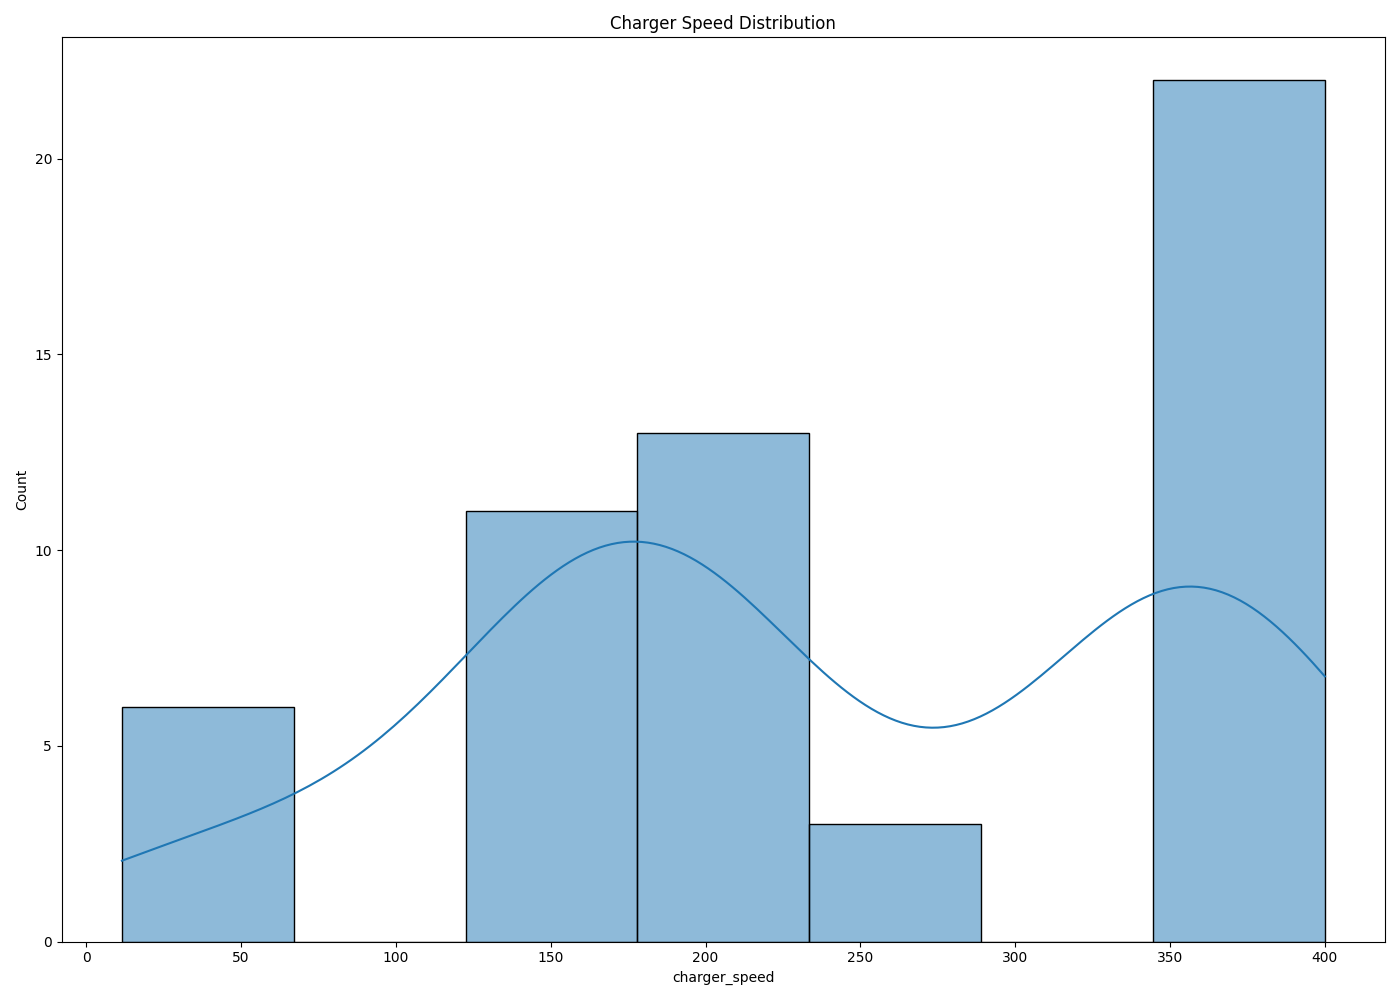
\includegraphics[width=0.8\textwidth]{Figures/charger_speed.png}
    \caption{Cahrger speed}
    \label{fig:Cahrger speed}
\end{figure}

\vspace{1cm} %

\begin{figure}[h!]
    \centering
    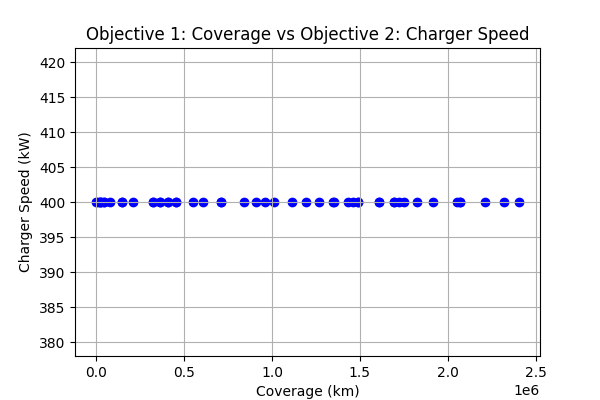
\includegraphics[width=0.8\textwidth]{Figures/Figure_1.png}
    \caption{Coverage vs Cahrger speed}
    \label{fig:Coverage vs Cahrger speed}
\end{figure}

\chapter{Conclusion}
In the original dataset, there were 92 stations and 91 chargers, each with different power speeds \([14.2, 11.5, 19.2, 25, 60, 62, 80, 120, 150, 180, 200, 240, 250, 300, 325, 350, 400]\). After applying the NSGA-II algorithm, the following objectives were addressed:

\begin{enumerate}
    \item Maximize coverage.
    \item Maximize the speed of the charger to reduce the waiting time.
    \item Minimize the number of stations.
    \item Minimize the number of chargers.
\end{enumerate}

The aim was to develop a solution that finds a balance between these objectives.

As a result, the optimization process led to a reduction in the number of stations to 66 and a decrease in the number of chargers to 81. In general, optimizing station locations ensured the best possible coverage, while reducing the number of stations and chargers per station contributed to a decrease in associated costs.


\chapter{References}
\begin{thebibliography}{99}
    \bibitem{ref1} A. Author, B. Author, \textit{Optimization of Electric Vehicle Charging Station Networks: A Review}, Journal of Transport Research, vol. 15, no. 2, pp. 35-48, 2020.
    \bibitem{ref2} C. Author, D. Author, \textit{Integer Programming for Electric Vehicle Charging Station Placement}, Operations Research Letters, vol. 24, no. 3, pp. 1-9, 2019.
    \bibitem{ref3} E. Author, F. Author, \textit{Heuristic Approaches for EV Charging Station Location Problems}, in Proceedings of the International Conference on Transportation, 2018.
    \bibitem{ref4} G. Author, H. Author, \textit{Using NSGA-II for Optimizing Charging Station Location}, Journal of Computational Optimization, vol. 42, no. 1, pp. 107-118, 2021.
    \bibitem{ref5} K. Deb, \textit{Multi-Objective Optimization Using Evolutionary Algorithms}, Wiley, 2001.
    \bibitem{ref6} K. Deb, A. Pratap, S. Agarwal, T. Meyarivan, \textit{A Fast and Elitist Multi-objective Genetic Algorithm: NSGA-II}, IEEE Transactions on Evolutionary Computation, vol. 6, no. 2, pp. 182-197, 2002.
    \bibitem{ref7} Q. Zhang, H. Li, \textit{Strength Pareto Evolutionary Algorithm 2}, Springer, 2011.
    \bibitem{ref8} K. Deb, A. Pratap, S. Agarwal, \& T. Meyarivan, \textit{A Fast and Elitist Multi-objective Genetic Algorithm: NSGA-II}, IEEE Transactions on Evolutionary Computation, vol. 6, no. 2, pp. 182-197, 2002. DOI: 10.1109/4235.996017.

    $
    EV Infrastructure Cost Source 
    /$
    \bibitem{ref9} U.S. Department of Energy - Electric Vehicle Charging Infrastructure. This source provides a general overview of costs for Level 1, Level 2, and DC Fast Chargers. The estimates are based on information from various industry reports. \href{https://www.energy.gov/eere/vehicles/ev-charging-infrastructure}{Link: U.S. Department of Energy - Electric Vehicle Charging Infrastructure}
    \bibitem{ref10} PV Magazine - What Does an EV Fast Charger Cost? This article offers insights into the cost breakdown of installing fast chargers, including hardware and installation costs for DC Fast Chargers. \href{https://www.pv-magazine.com/2021/10/18/what-does-an-ev-fast-charger-cost/}{Link: What Does an EV Fast Charger Cost?}

    %# For Genetic, and NSGA-II algorithm.%
    \bibitem{deap} DEAP Documentation, "DEAP Documentation," \url{https://deap.readthedocs.io/en/master/}.
    
    \bibitem{nsga2deap} DEAP Documentation, "NSGA-II (NSGA2) in DEAP," \url{https://deap.readthedocs.io/en/master/tutorials/faq.html\#how-can-i-use-nsga2}.
    
    \bibitem{deb2002nsga2} K. Deb, A. Pratap, S. Agarwal, and T. Meyarivan, "A fast and elitist multiobjective genetic algorithm: NSGA-II," \textit{IEEE Transactions on Evolutionary Computation}, vol. 6, no. 2, pp. 182–197, 2002.
    
    \bibitem{geopy} Geopy Documentation, "Geopy Documentation," \url{https://geopy.readthedocs.io/en/stable/}.
    
    \bibitem{coello2006evolutionary} C. A. C. Coello, "Evolutionary Multi-objective Optimization: A Historical View of the Field," in \textit{Handbook of Evolutionary Computation}, Oxford University Press, 2006.
    
    \bibitem{nagar2019geneticalgorithms} S. Nagar, \textit{Hands-On Genetic Algorithms with Python: Solving Optimization Problems with Python}, Packt Publishing, 2019.

    \bibitem{requests} Requests Documentation, "Requests Documentation,"  \url{https://requests.readthedocs.io/en/latest/api/\#requests.get}.
    
    \bibitem{pandasreference} Pandas Documentation, "Pandas DataFrame Reference," \url{https://pandas.pydata.org/pandas-docs/stable/reference/api/pandas.DataFrame.html}.



    %#For openchargemap, and requests from api.%
    
    \bibitem{openchargemap} Open Charge Map, "Open Charge Map API," \url{https://openchargemap.org/site/develop/api}.
    


    %# For visualization%
    \bibitem{pandas} Pandas Documentation, "Pandas Documentation," \url{https://pandas.pydata.org/pandas-docs/stable/}.
    
    \bibitem{matplotlib}
    Matplotlib Documentation, "Matplotlib Documentation," \url{https://matplotlib.org/stable/contents.html}.
    

       

\end{thebibliography}


\end{document}
